% !TEX root =./main.tex

\section{Signal $x_7$}

Finally, Signal $x_7$ consists of 10 test tones, each separated by $1000 \unit{Hz}$.  The processing goal of this signal is to make the magnitudes of the test tones rest within $1 \unit{dB}$ of the brown line in Figure \ref{fig:X7}.

\begin{figure}[H]
    \centering
    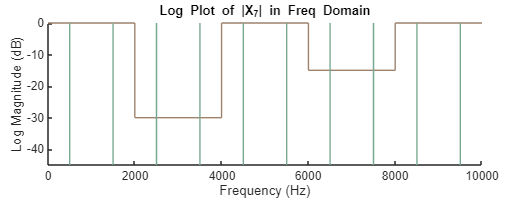
\includegraphics[width=0.5\linewidth]{figures/X7_prefilter.png}
    \caption{Frequency Spectrum of Signal $x_4$ with Desired Magnitude Line}
    \label{fig:X7}
\end{figure}

In order to create the necessary filter, we will use the \code{firpm} function, which implements the Remez algorithm to interpolate given points in a way that minimizes the maximum error.  This interpolation then is converted into a filter.  

In order to make the best use of this feature, we will use the frequencies of the test tones coupled with the desired magnitudes as the points given to the \code{firpm} function.  This can be seen in Figure \ref{fig:x7_filterResponse}, where the red x's represent the points given to the \code{firpm} function.  After trying every order working up from order 3, Matlab's minimum filter order, order 50 was determined to be the first to meet these requirements.  Filter 1's frequency response can be seen in blue.

\begin{figure}[H]
    \centering
    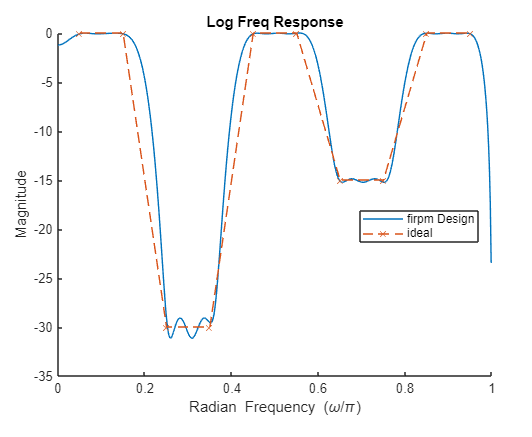
\includegraphics[width=0.5\linewidth]{figures/x7_filterdesign.png}
    \caption{Frequency Response of Filter 1 for Signal $x_7$}
    \label{fig:x7_filterResponse}
\end{figure}

These points are listed in Table \ref{tab:x7_filter1}.

\begin{table}[H]
    \centering
    \begin{tabular}{cc}
        Normalized Angular Frequency & Magnitude \\ \hline
        0.05 & 1.0\\
        0.15 & 1.0\\
        0.25 & 0.031623\\
        0.35 & 0.031623\\
        0.45 & 1.0\\
        0.55 & 1.0\\
        0.65 & 0.17783\\
        0.75 & 0.17783\\
        0.85 & 1.0\\
        0.95 & 1.0
    \end{tabular}
    \caption{Parameters for Filter 1 for Signal $x_7$}
    \label{tab:x7_filter1}
\end{table}

Applying Filter 1 to Signal $x_7$ yields the frequency response in Figure \ref{fig:x7_filtered}, where it can be seen that all tones are very close to the desired magnitude line.

\begin{figure}[H]
    \centering
    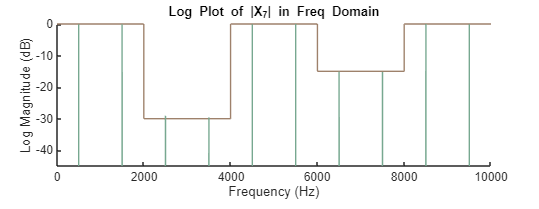
\includegraphics[width=0.5\linewidth]{figures/x7_postfilter.png}
    \caption{Response of Signal $x_4$ to Filter 1, Order 50}
    \label{fig:x7_filtered}
\end{figure}

The errors at each tone are compiled in Table \ref{tab:x7_errors}

\begin{table}[H]
    \centering
    \begin{tabular}{cc}
        Frequency (Hz) & Error \\ \hline
        500  & 0.06762\\
        1500 & 0.06377\\
        2500 & 0.93816\\
        3500 & 0.39825\\
        4500 & 0.06582\\
        5500 & 0.00000 \\
        6500 & 0.10854\\
        7500 & 0.22556\\
        8500 & 0.00107\\
        9500 & 0.06390
    \end{tabular}
    \caption{Errors for Tones in Signal $x_7$}
    \label{tab:x7_errors}
\end{table}

\vspace{-2pt}

From this, we can see that the maximum error is $0.93816$, and so every tone is within the $1 \unit{dB}$ tolerance that is required.  We can also calculate that the mean error is $0.1932 \unit{dB}$.  

However, notice that the Remez algorithm minimizes the maximum absolute difference between the polynomial and the function, but does not minimize the maximum absolute error at each of the given points.  Thus, \code{firpm} minimizes the error off the of the dashed red line in Figure \ref{fig:x7_filterResponse}, but does not ensure that the polynomial passes through every point.  In this application, because we are primarily interested in the values at the 10 test tones, if we instead used a method such as Lagrange polynomial interpolation or cubic spline polynomial interpolation, we could get the required error with a much lower order.